\newcommand{\showListItem}[1]{\item #1}

\newenvironment{sritiesGerinimas}[1]
{
% Exposed commands
\newcommand{\vertinimas}[2]{\gdef\SritiesOld{##1} \gdef\SritiesNew{##2}}
\newcommand{\veiksmas}[1]{\listgadd{\SritiesVeiksmai}{##1}}
\newcommand{\argumentacija}[1]{\gdef\SritiesArgumentacija{##1}}

% Internal defs

\def\Name{#1}
\def\SritiesOld{}
\def\SritiesNew{}
\def\SritiesVeiksmai{}
\def\SritiesArgumentacija{}

% Beginning
\subsubsection{\Name}\label{sec:gerinimas:\Name}
}{
% Ending
Keliamas \textit{\Name}~gebėjimo lygis: \textbf{\SritiesOld} $\rightarrow$ \textbf{\SritiesNew}
\begin{itemize}
    \forlistloop{\showListItem}{\SritiesVeiksmai}
\end{itemize}
\SritiesArgumentacija{}
}

\newenvironment{tiksloGerinimas}[1]
{
% Exposed commands
\renewcommand{\vertinimas}[2]{\gdef\TiksloOld{##1} \gdef\TiksloNew{##2}}
\renewcommand{\veiksmas}[1]{\listgadd{\TiksloVeiksmai}{##1}}
\renewcommand{\argumentacija}[1]{\gdef\TiksloArgumentacija{##1}}

% Internal defs

\def\Name{#1}
\def\TiksloOld{}
\def\TiksloNew{}
\def\TiksloVeiksmai{}
\def\TiksloArgumentacija{}
% Beginning
}{
% Ending
\textit{\Name}~specifinis tikslas: \textbf{\TiksloOld} $\rightarrow$ \textbf{\TiksloNew}
\begin{itemize}
    \forlistloop{\showListItem}{\TiksloVeiksmai}
\end{itemize}
\TiksloArgumentacija{}
}

\newenvironment{praktikosGerinimas}[1]
{
% Exposed commands
\renewcommand{\vertinimas}[2]{\gdef\PraktikosOld{##1} \gdef\PraktikosNew{##2}}
\renewcommand{\veiksmas}[1]{\listgadd{\PraktikosVeiksmai}{##1}}
\renewcommand{\argumentacija}[1]{\gdef\PraktikosArgumentacija{##1}}
% Internal defs

\def\Name{#1}
\def\PraktikosOld{}
\def\PraktikosNew{}
\def\PraktikosVeiksmai{}
\def\PraktikosArgumentacija{}
% Beginningme
}{
% Ending
\textit{\Name}~specifinė praktika: \textbf{\PraktikosOld} $\rightarrow$ \textbf{\PraktikosNew}
\ifdefempty{\PraktikosVeiksmai}{\\}{
\begin{itemize}
    \forlistloop{\showListItem}{\PraktikosVeiksmai}
\end{itemize}
}
\PraktikosArgumentacija{}
}
\section{Gerinimas}
\subsection{Tikslinis profilis}
\begin{figure}[h]
    \centering
    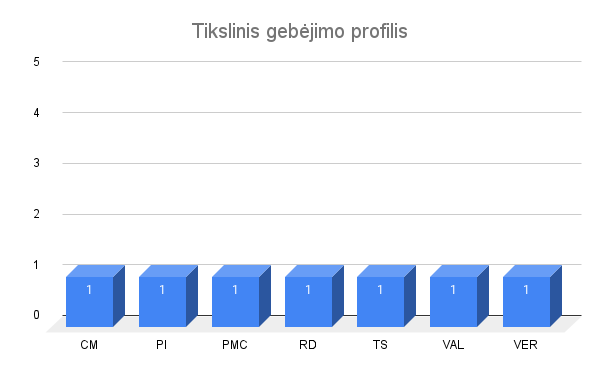
\includegraphics[width=0.75\linewidth]{gerinimas//img/tikslinis.png}
\end{figure}
\subsection{Gerinimo veiksmų planas}
% RD
\begin{sritiesGerinimas}{Requirements Development}
    \vertinimas{0}{1}
    \veiksmas{
        \begin{tiksloGerinimas}{RD.SG 2 Develop Product Requirements}
        \vertinimas{Unsatisfied}{Satisfied}
        \veiksmas{
            \begin{praktikosGerinimas}{RD.SP 2.3 Identify Interface Requirements}
                \vertinimas{NI}{FI}
                \veiksmas{
                    Reikalavimų analizės (RA) procese pridėti naują veiklą:
                    \hladd {
                        Analitikas identifikuoja išorines sąsajas su kuriomis turės komunikuoti kuriama sistema. 
                    }
                }
                \veiksmas{
                    Reikalavimų analizės (RA) procese pridėti naują veiklą:
                    \hladd{
                        Architektas analizuoja identifikuotas išorines sąsajas ir rašo (ISD). 
                    }
                }
                \veiksmas{
                    Pridėti naują darbo produktą:
                    \hladd{
                        \textbf{ISD} - Išorinių Sąsajų Dokumentacija. Šioje dokumentacijoje yra aprašyta visos aktualios išorinių sąsajų techninės detalės, kurių gali prireikti kuriant integracija su šiomis sąsajomis.
                    }
                }
                \veiksmas{
                    Reikalavimų analizės (RA) procese atnaujinti veiklą (2):
                    \hladd{
                        Architektas ir analitikas apibrėžia funkcinius (FR) ir nefunkcinius reikalavimus (NFR) iš identifikuotų naudotojų poreikių, modeliuojamų verslo procesų, projekto apimties (PA) ir identifikuotų išorinių sąsajų.
                    }
                }
                \veiksmas{
                    Įgyvendinimo (ĮG) atnaujinti veiklą (5):
                    \hladd{
                        Kiekvienas programinės įrangos kūrėjas rašo kodą, jei prireikia, naudoja išorinių sąsajų dokumentaciją (ISD), kad įgyvendintų priskirtą užduotį ir taip papildo programinį kodą (PK).
                    }
                }
                \argumentacija{Šie pakeitimai užtikrins, kad analizės metu informacija apie išorines sąsajas bus surinkta ir panaudota.}
            \end{praktikosGerinimas}
        }
        \argumentacija{
            Atlikus pakeitimus, reikalavimų rengimas bus pakankamai kontroliuojamas, jog likę trūkumai (reikalavimų priklausomybių neatnaujinimas keičiantis reikalavimams) nebūtų esminiai. Todėl specifinis tikslas laikomas pasiektu (\textbf{Satisfied})
        }
        \end{tiksloGerinimas}
    }
    \veiksmas{
        \begin{tiksloGerinimas}{RD.SG 3 Analyze and Validate Requirements}
        \vertinimas{Unsatisfied}{Satisfied}
        \veiksmas{
            \begin{praktikosGerinimas}{RD.SP 3.3 Analyze Requirements}
                \vertinimas{PI}{LI}
                \veiksmas{
                    Reikalavimų analizės (RA) procese atnaujinti veiklą (1): 
                    \hladd{Analitikas renka informaciją iš kliento. Pagal tai modeliuoja verslo procesus ir identifikuoja konkrečius naudotojų poreikius. Jei kyla prieštaraujančių reikalavimų - sprendžia juos su atitinkamais SŠ. }
                }
                \veiksmas{
                    Reikalavimų analizės (RA) procese pridėti veiklą: 
                    \hladd{Analitikas daro analizę, bendrauja su SŠ, aiškinasi ar reikalavimų rinkinys yra pilnas ir būtinas. Jei pasirodo, kad rinkinys yra ne pilnas grįžtama prie pirmos veiklos.}
                }
                \veiksmas{
                    Reikalavimų analizės (RA) procese pridėti veiklą: 
                    \hladd{Analitikas ir architektas atlieka analizę, aiškinasi ar iškelti funkciniai (FR) ir nefunkciniai (NFR) reikalavimai yra įgyvendinami ir patikrinami. Jei pasirodo, kad rinkinyje yra neįgyvendinamų arba nepatikrinamų reikalavimų, jie yra performuluojami. }
                }
                \veiksmas{
                    Reikalavimų analizės (RA) procese pridėti veiklą: 
                    \hladd{Analitikas, architektas ir programinės įrangos kūrėjai ruošia sistemos maketą, kuris atitiktų surinktų funkcinių (FR) ir nefunkcinių (NFR) reikalavimų rinkinį. }
                }
                \veiksmas{
                    Reikalavimų analizės (RA) procese pridėti veiklą: 
                    \hladd{Analitikas ir Architektas pristato SŠ maketą, aiškinasi su SŠ ar reikalavimų rinkinys yra pakankamas. Jei SŠ turi kritinių pastabų, procesas yra kartojamas.}
                }
                \argumentacija{Šie pakeitimai užtikrins, kad analizės metu surinkti reikalavimai atitiktų klientų poreikius ir įgyvendins specifinės praktikos subpraktikas (1-3), tačiau išlieka trūkumai, kad nėra nustatoma, kokie techniniai indikatoriai bus sekami ir kad detalios koncepcijos yra kuriamos pabaigus vykdyti visas projekto užduotis todėl, jos negali būti analizuojamos norint atrasti naujų reikalavimų. }
            \end{praktikosGerinimas}
        }
        \veiksmas{
            \begin{praktikosGerinimas}{RD.SP 3.4 Analyze Requirements to Achieve Balance}
                \vertinimas{PI}{LI}
                \veiksmas{
                   
                }
                \argumentacija{Praeitos specifinės praktikos gerinimas įvykdo šios specifinės praktikos sub-praktiką (1) - yra naudojami modeliai norint išgauti informaciją apie reikalavimus. Tačiau dar išlieka trūkumų: produkto gyvavimo ciklo koncepcijos nėra sudaromos, nėra analizuojamos ir architektūrą lemiančios patogumo funkcijos, jų poveikis projekto kainai ir rizika nėra analizuojamos.}
            \end{praktikosGerinimas}
        }
        \veiksmas{
            \begin{praktikosGerinimas}{RD.SP 3.5 Validate Requirements}
                \vertinimas{NI}{LI}
                \veiksmas{
                   Reikalavimų analizės (RA) procese pridėti veiklą: 
                    \hladd{Analitikas atlieka rizikos analizę. Yra analizuojama poveikis produktui, jei įgyvendinimo metu pasirodytų, kad tam tikri reikalavimai negali būti išpildyti. }
                }
                \argumentacija{Užpraeitos specifinės praktikos gerinimas įvykdo šios specifinės praktikos sub-praktiką (2) - kuriami sistemos prototipai. Nauja veikla užtikrina, kad rizika bus įvertinta, jei pasirodytų, kad tam tikri reikalavimai negali būti išpildyti. Išlieka trūkumas - bręstantis sistemos dizainas nėra analizuojamas reikalavimų kontekste}
            \end{praktikosGerinimas}
        }
        \argumentacija{Atlikus pakeitimus, reikalavimų rengimas bus pakankamai kontroliuojamas, jog likę trūkumai nebūtų esminiai. Todėl specifinis tikslas laikomas pasiektu (\textbf{\TiksloNew}).}
        \end{tiksloGerinimas}
    }
    \argumentacija{Atlikus šiuos pakeitimus, visi \Name~specifiniai tikslai bus įvertinti kaip \textbf{Satisfied}, todėl proceso srities gebėjimo lygis pakils iki \textbf{\SritiesNew}}
\end{sritiesGerinimas}
% -------------------------------------------------------------
% VER
\begin{sritiesGerinimas}{Verification}
    \vertinimas{0}{1}
    \veiksmas{
        \begin{tiksloGerinimas}{VER.SG 1 Prepare for Verification}
        \vertinimas{Unsatisfied}{Satisfied}
        \veiksmas{
            \begin{praktikosGerinimas}{VER.SP 1.3 Establish Verification Procedures and Criteria}
                \vertinimas{NI}{FI}
                \veiksmas{
                    Kontrolės (KO) procese atnaujinti veiklą (5):
                    \hladd{
                        Remiantis komandos atsiliepimais, komanda ir projektų vadovas nustato komandos procesų pakeitimus, kurie įsigalioja nuo kito sprinto. Pakeitimai gali įtraukti naujas verifikacijos procedūras darbo produktams, jų priėmimo kriterijų naujinimus, kriterijų vertinimo slenkstines ribas.
                    }
                }
                \argumentacija{Šie pakeitimai užtikrins, kad būtų vystomos ir palaikomos verifikavimo procedūros atitinkamiems darbo produktams.}
            \end{praktikosGerinimas}
        }
        \argumentacija{Atlikus pakeitimus, pasiruošimo verifikacijai veiksmai bus pakankamai kontroliuojami, jog likę trūkumai nebūtų esminiai. Todėl specifinis tikslas laikomas pasiektu (\textbf{\TiksloNew}).}
        \end{tiksloGerinimas}
    }
    \veiksmas{
        \begin{tiksloGerinimas}{VER.SG 2 Perform Peer Reviews}
        \vertinimas{Unsatisfied}{Satisfied}
        \veiksmas{
            \begin{praktikosGerinimas}{VER.SP 2.3 Analyze Peer Review Data}
                \vertinimas{NI}{LI}
                \veiksmas{
                    Pridėti naują darbo produktą:
                    \hladd{
                        \textbf{KPR} - Kodo Peržiūros Raportas. Šiame dokumente renkama informacija apie pasiruošimą kodo peržiūrai, jos eigą ir rezultatus.
                    }
                }
                \veiksmas{
                    Įgyvendinimo (RA) procese atnaujinti veiklą (9): 
                    \hladd{
                        Užduotį, kuri yra IN REVIEW, kitas komandos narys peržiūri, komentuoja kodą. Tas pats komandos narys užpildo kodo peržiūros raportą (KPR).  Jeigu kitas komandos narys pareikalauja pakeitimų, pakeičia užduoties statusą į IN PROGRESS. Už užduotį atsakingas asmuo turi pakartoti 7-9 veiklas.
                    }
                }
                \veiksmas{
                    Projekto Užbaigimo (PU) procese pridėti veiklą (9): 
                    \hladd{
                        Analitikas atlieka kodo peržiūros raportų (KPR) analizę, identifikuoja pasikartojančias problemas ir bendro susitikimo metu jas adresuoja su kitais komandos nariais, taip prisidedama prie departamento patirties (PAT) ugdymo.
                    }
                }
                \argumentacija{Šie pakeitimai užtikrins, kad kodo peržiūros duomenys yra renkami ir analizuojami.}
            \end{praktikosGerinimas}
        }
        \argumentacija{Atlikus pakeitimus, peržiūros veiksmai bus pakankamai kontroliuojami, jog likę trūkumai (neužtikrinama, kad peržiūros duomenys nebūtų naudojami netinkamai) nebūtų esminiai. Todėl specifinis tikslas laikomas pasiektu (\textbf{\TiksloNew}).}
        \end{tiksloGerinimas}
    }
    \argumentacija{Atlikus šiuos pakeitimus, visi \Name~specifiniai tikslai bus įvertinti kaip \textbf{Satisfied}, todėl proceso srities gebėjimo lygis pakils iki \textbf{\SritiesNew}}
\end{sritiesGerinimas}
\newpage

Project monitoring and control
\begin{sritiesGerinimas}{Project monitoring and control}
    \vertinimas{0}{1}
    \veiksmas{

        \begin{tiksloGerinimas}{SG 1 Monitor the Project Against the Plan}
        \vertinimas{Unsatisfied}{Satisfied}
        \veiksmas{

            \begin{praktikosGerinimas}{Monitor Stakeholder Involvement}
                \vertinimas{NI}{FI}
                \veiksmas{
                    Pridėti naują darbo produktą: 
                    \hladd{
                        \textbf{SŠĮA} -- Suinteresuotų šalių įsitraukimo ataskaita. Čia aprašomas SŠ įsitraukimas, susįjusios problemos ir jų pasekmės ir galimi sprendimo būdai.
                    }
                }
                \veiksmas{
                    Pristatymo ir grįžtamojo ryšio surinkimo (PAS) procese pridėti veiklą: 
                    \hladd{
                        Projekto vadovas peržiūti suinteruotų šalių įsitraukimą. Jeigu kyla problemų, atlieka analizę ir nustato jų poveikį. Tai, projektų vadovas, surašo suinteresuotų šalių įsitraukimo ataskaitoje.
                    }
                }
                \veiksmas{Kontrolės (KO) procese pakeisti 3 veiklą:
                    Projekto vadovas vykdo stebėseną ir esant reikalui švelnina rizikas arba vykdo žalos kontrolę pagal rizikų valdymo planą (RVP) \hladd{ir suinteresuotų šalių įsitraukimo ataskaitą (SŠĮA).}
                    }
                \argumentacija{Šie pakeitimai užtikrina, kad vyskta SŠ įsitraukimo kontrolė bei kad SŠ įsitraukimo kontrolės rezultatai yra dokumentuojami.}
            \end{praktikosGerinimas}

            \begin{praktikosGerinimas}{Conduct Progress Reviews}
                \vertinimas{PI}{LI}
                \veiksmas{Kontrolės (KO) procese pakeisti 3 veiklą:
                    \hladd{Analitikas analizuoja naują informaciją iš komandos narių atsiliepimų ir grįžtamojo ryšio registro, įvertina ar nepasikeitė esamos ir/ar neatsirado naujos projekto rizikos, pagal tai analizuoja rizikas ir atnaujina rizikų valdymo planą (RVP).}
                    Projekto vadovas vykdo stebėseną ir esant reikalui švelnina rizikas arba vykdo žalos kontrolę pagal rizikų valdymo planą (RVP) \hladd{, papildomai informuodamas atitinkamas SŠ.}
                    }
                \argumentacija{Šie pakeitimai užtikrina, kad rizikos yra nuolat analizuojamos, reaguojama į naują informaciją ir rizikas, taip pat informuojamos SŠ.}
            \end{praktikosGerinimas}

            \begin{praktikosGerinimas}{Monitor Project Planning Parameters}
                \vertinimas{PI}{LI}
                \veiksmas{Kontrolės (KO) procese pridėti veiklą:
                        Projekto vadovas peržiūri sprinto užduočių sąrašą (SUS), į jį atsižvelgdamas, palygina faktinį užduotims skirtus žmogiškuosius išteklius su pradinėmis sąmatomis (IS), pagal tai paskaičiuoja kainos ir įdėtų pastangų ataskaitą.
                    }
                \veiksmas{Kontrolės (KO) procese pakeisi veiklą 4:
                    Remiantis grįžtamojo ryšio registru (GRR)\hladd{, kainos ir įdėtų pastangų ataskaita} ir laiko valdymo ataskaita projekto vadovas atlieka projekto užduočių sąrašo (PUS) atnaujinimą, prireikus, užduočių prioritetų keitimą, pasakojimo vienetų intervalo (PVI) patikslinimą. Šie pakeitimai fiksuojami sprinto peržiūros ataskaitoje (SPA).
                }
                \argumentacija{Šie pakeitimai užtikrina, kad bus sekama kaina ir pastangos.}
            \end{praktikosGerinimas}

            \begin{praktikosGerinimas}{Conduct Progress Reviews}
                \vertinimas{PI}{LI}
                \veiksmas{Įgyvendinimo (ĮG) procese pakeisti veiklą 1:
                    Kiekvieną dieną komanda rengia trumpą Stand-Up susitikimą, kad aptartų progresą, nustatytu kliūtis ir sinchronizuotu ̨ veiklas tarp komandos narių. Šis susitikimas įprastai trunka ne ilgiau kaip 15 minučių ir susideda iš trijų pagrindinių punktų: kas buvo padaryta vakar, kas bus daroma šiandien, ir su kokiomis kliūtimis susiduriama.
                    \hladd{Projekto vadovas atsižvelgdamas į kliutis, jeigu reikia, atitinkamai pakeičia sprinto užduočių sąrašą (SUS).}
                }
                \argumentacija{TODO}
            \end{praktikosGerinimas}
            
        }
        \end{tiksloGerinimas}

%%%%%%%%%%%%%%%%%%%%%%%%%%%%%%%%%%%%%%%%%%%%%%%%%%%%%%%%%%%%%%%%%%%

        \begin{tiksloGerinimas}{PMC.SG 2 Manage Corrective Action to Closure}
        \vertinimas{Unsatisfied}{Satisfied}
        \veiksmas{
            \begin{praktikosGerinimas}{Take Corrective Action}
                \vertinimas{PI}{LI}
                \veiksmas{Kontrolės (KO) procese pakeisti 3 veiklą:
                    Projekto vadovas vykdo stebėseną ir esant reikalui švelnina rizikas arba vykdo žalos kontrolę pagal rizikų valdymo planą, \hladd{prieš tai peržiūrėdamas paveiktas SŠ ir gaudamas leidimą iš jų}.
                }
                \argumentacija{Šie pakeitimai užtikrina, kad gaunamas sutikimas švelninti rizikas arba vykdyti žalos kontrolę, gaunant sutikimą iš SŠ}
            \end{praktikosGerinimas}
        }
        \vertinimas{Unsatisfied}{Satisfied}
        \veiksmas{
            \begin{praktikosGerinimas}{Manage Corrective Actions}
                % 1. Monitor corrective actions for their completion. 
                % 2. Analyze results of corrective actions to determine the effectiveness of the corrective actions. 
                \vertinimas{PI}{LI}
                \veiksmas{Kontrolės (KO) procese pakeisti 3 veiklą:
                    Projekto vadovas vykdo stebėseną ir esant reikalui švelnina rizikas arba vykdo žalos kontrolę pagal rizikų valdymo planą (RVP) \hladd{, papildant rizikų valdymo planą koregavimo veiksmų eigos statusu}.
                }
                \veiksmas{Kontrolės (KO) procese pridėti veiklą:
                    Projekto vadovas peržiūri visų koregavimo veiksmų statusus. Peržiūri ar visi koregavimo veiksmai buvo tinkami ir pasiekė savo tikslą.
                }
                \argumentacija{Šie pakeitimai užtikrina, kad koregavimo veiksmai yra ne tik tinkamai stebimi, bet ir vertinamas jų veiksmingumas.}
            \end{praktikosGerinimas}
        }
        \end{tiksloGerinimas}
    }
\end{sritiesGerinimas}

\newpage
\begin{sritiesGerinimas}{Technical solution}
    \vertinimas{0}{1}
    \veiksmas{

        \begin{tiksloGerinimas}{SG 1 Select Product Component Solutions}
        \vertinimas{Unsatisfied}{Satisfied}
        \veiksmas{

            \begin{praktikosGerinimas}{Develop Alternative Solutions and Selection Criteria}
                \vertinimas{PI}{LI}
                \veiksmas{Reikalavimų analizės (RA) procese pridėti veiklą:
                    \hladd{Architektas ieško naujų technologijų ir COTS produktų, kuriuos galėtų panaudoti projekte, jeigu tokius atranda, papildo aukšto lygio architektūrą (ALSA).}
                }
                \argumentacija{Šis pakeitimas, jog atsižvelgiama į COTS produktus ir naujas technologijas, kurias būtų galima panaudoti projekte.}
            \end{praktikosGerinimas}
        }
        \end{tiksloGerinimas}
    }
\end{sritiesGerinimas}
\begin{sritiesGerinimas}{Configuration Management}
    \vertinimas{0}{1}
    \veiksmas{
        \begin{tiksloGerinimas}{CM.SG 1 Establish Baselines}
        \vertinimas{Unsatisfied}{Satisfied}
        \veiksmas{
            \begin{praktikosGerinimas}{CM.SP 1.2 Establish a Configuration Management System}
                \vertinimas{NI}{LI}
                \veiksmas{
                    Pridėti naują darbo produktą: 
                    \hladd{
                        \textbf{KFR} -- Konfigūracinių Failų Repozitorija. Čia laikomi produkto konfigūraciniai failai. Pagrindinė šios repozitorijos šaka atitinka bazinę produkto konfigūraciją.
                    }
                }
                \veiksmas{
                    Aplinkos rengimo (AR) procese pridėti veiklą: 
                    \hladd{
                        Architektas sukuria produkto konfigūracinių failų repozitoriją (KFR) ir parengia ją naudojimui.
                    }
                }
                \argumentacija{Šie pakeitimai užtikrins, jog konfigūracijos valdymas yra atskirtas nuo kodo ir atitinka 3--9 detaliąsias praktikas pasirinktai konfigūracijos valdymo strategijai. Tačiau išlieka autorizacijos lygių atskyrimo trūkumas, todėl specifinės praktikos įvertinimas keliamas iki \textbf{\PraktikosNew}.}
            \end{praktikosGerinimas}
        }
        \argumentacija{Atlikus pakeitimus, visos specifinės praktikos įgyja \textbf{LI} įvertinimą, o trūkumai (neatskirti kontrolės lygiai ir nesudaryta CCB) nedaro esminio poveikio specifiniam tikslui. Todėl specifinis tikslas laikomas pasiektu (\textbf{\TiksloNew})}
        \end{tiksloGerinimas}
    }
    \veiksmas{
        \begin{tiksloGerinimas}{CM.SG 2 Track and Control Changes}
        \vertinimas{Unsatisfied}{Satisfied}
        \veiksmas{
            \begin{praktikosGerinimas}{CM.SP 2.2 Control Configuration Items}
                \vertinimas{LI}{FI}
                \veiksmas{
                    Aplinkos rengimo (AR) procese pridėti veiklą: 
                    \hladd{
                        Architektas užtikrina, jog konfigūracinių failų repozitorijos (KFR) pagrindinė šaka būtų atnaujinama tik kai pakeitimą patvirtina Projekto Vadovas.
                    }
                }
                \argumentacija{Po šio pakeitimo naują bazinę konfigūraciją turės patvirtinti (autorizuoti) Projekto Vadovas, įsitikinęs, jog su šiuo pakeitimu sutinka visos SŠ, todėl specifinės praktikos įvertinimas pakils iki \textbf{\PraktikosNew}.}
            \end{praktikosGerinimas}
        }
        \argumentacija{Atlikus pakeitimus, konfigūracijos valdymas bus pakankamai kontroliuojamas, jog likę trūkumai (nepakankamas pakeitimų matomumas visoms SŠ) nebūtų esminiai. Todėl specifinis tikslas laikomas pasiektu (\textbf{\TiksloNew}).}
        \end{tiksloGerinimas}
    }
    \veiksmas{
        \begin{tiksloGerinimas}{CM.SG 3 Establish Integrity}
        \vertinimas{Unsatisfied}{Satisfied}
        \veiksmas{
            \begin{praktikosGerinimas}{CM.SP 3.1 Establish Configuration Management Records}
                \vertinimas{NI}{LI}
                \argumentacija{\\
                    Atlikus aukščiau \ref{sec:gerinimas:Configuration Management} aprašytus pakeitimus, įgyvendinamos visos \Name~detaliosios praktikos, išskyrus pakankamą konfigūracijos valdymo matomumą visoms SŠ, todėl specifinė praktika įgyja \textbf{\PraktikosNew} įvertinimą.
                }
            \end{praktikosGerinimas}
        }
        \veiksmas{
            \begin{praktikosGerinimas}{CM.SP 3.2 Perform Configuration Audits}
                \vertinimas{NI}{FI}
                \veiksmas{Sukurti naują periodiškai iki projekto pabaigos vykstantį procesą \hladd{Projekto Konfigūracijos Auditas (KAU)} ir jame pridėti toliau išdėstytas veiklas.}
                \veiksmas{\hladd{
                    Palyginama konfigūracijos repozitorijoje (KFR) esanti bazinė konfigūracija su techninėje dokumentacijoje (TD) aprašyta konfigūracija.
                }}
                \veiksmas{\hladd{
                    Patikrinama, ar visi konfigūracijos nustatymai turi tinkamus identifikatorius ir yra minimi techninėje dokumentacijoje (TD).
                }}
                \veiksmas{\hladd{
                    Patikrinama konfigūracijos repozitorijos (KFR) pakeitimų istorija ir užtikrinama, jog visi pakeitimai dokumentuoti ir susieti su projekto užduotimis, esančiomis projekto užduočių sąraše (PUS).
                }}
                \veiksmas{\hladd{
                    Jei rasta neatitikimų, jie užregistruojami kaip atskiros užduotys projekto užduočių sąraše (PUS).
                }}
                \argumentacija{Atlikus šiuos pakeitimus bus atliekamas konfigūracijos auditas pritaikytas pasirinktai konfigūracijos valdymo strategijai ir išpildantis detaliąsias praktikas. Todėl specifinė praktika įgyja \textbf{\PraktikosNew} įvertinimą.}
            \end{praktikosGerinimas}
        }
        \argumentacija{Atlikus pakeitimus, visų tikslo specifinių praktikų įvertinimai bus $\ge$ \textbf{LI}, o likę trūkumai (nepakankamas konfigūracijos valdymo matomumas visoms SŠ) nedarys esminio poveikio specifiniam tikslui. Todėl specifinis tikslas laikomas pasiektu (\textbf{\TiksloNew}).}
        \end{tiksloGerinimas}
    }
    \argumentacija{Atlikus šiuos pakeitimus, visi \Name~specifiniai tikslai bus įvertinti kaip \textbf{Satisfied}, todėl proceso srities gebėjimo lygis pakils iki \textbf{\SritiesNew}}
\end{sritiesGerinimas}
% -------------------------------------------------------------------------------
\begin{sritiesGerinimas}{Product Integration}
    \vertinimas{0}{1}
    \veiksmas{
        \begin{tiksloGerinimas}{PI.SG 2 Ensure Interface Compatibility}
        \vertinimas{Unsatisfied}{Satisfied}
        \veiksmas{
            \begin{praktikosGerinimas}{PI.SP 2.1 Review Interface Descriptions for Completeness}
                \vertinimas{PI}{FI}
                \veiksmas{
                    Pridėti veiklą Kontrolės (KO) procese: 
                    \hladd{
                        Architektas peržiūri techninėje dokumentacijoje (\textit{TD}) aprašytas vidines ir išorines produkto (\textit{PROD}) sąsajas ir, jei reikia, atnaujina projekto užduočių sąrašą (\textit{PUS}) pridėdamas į jį reikalingas sąsajų atnaujinimo veiklas.
                    }
                }
                \argumentacija{
                    Po šio pakeitimo architektas periodiškai peržiūrės produkto sąsajas užtikrindamas jų pilnumą ir jų apibrėžimų korektiškumą. Trūkumų nelieka, todėl šios specifinės praktikos įvertinimas pakyla iki \textbf{\PraktikosNew}.
                }
            \end{praktikosGerinimas}
        }
        \argumentacija{
            Atlikus šiuos pakeitimus, visos specifinio tikslo praktikos turės įvertinimą $\ge$ \textbf{LI}, o likę nustatyti trūkumai (sąsajų suderinamumo užtikrinimas tik \textit{SDLC}, o ne \textit{SLC} metu) neturės esminio poveikio.
        }
        \end{tiksloGerinimas}
    }
    \argumentacija{Atlikus šiuos pakeitimus, visi \Name~specifiniai tikslai bus įvertinti kaip \textbf{Satisfied}, todėl proceso srities gebėjimo lygis pakils iki \textbf{\SritiesNew}}
\end{sritiesGerinimas}
\begin{sritiesGerinimas}{Requirements Management}
    \vertinimas{0}{1}
    \veiksmas{
        \begin{tiksloGerinimas}{REQM.SG 1 Manage Requirements}
        \vertinimas{Unsatisfied}{Satisfied}
        \veiksmas{
            \begin{praktikosGerinimas}{REQM.SP 1.1. Understand Requirements}
                \vertinimas{PI}{LI}
                \veiksmas{Sukuriamas naujas produktas: 
                \hspace*{1cm}\newline Id:
                \hladd{KR}
                \hspace*{1cm}\newline Pavadinimas:
                \hladd{Kliento reikalavimai projektui}
                \hspace*{1cm}\newline Aprašymas:
                \hladd{
                Kliento pusėje suprojektuoti reikalavimai projektui, kurie apibrėžia detales, kaip kliento poreikiai projektui (KP) turėtų būti išpildyti projekte. 

                Kliento poreikių projektui (KP) dokumentas apima techninius, kokybinius, ir veikimo reikalavimus, reikalingus projekto sėkmei užtikrinti. 
                %Reikalavimų kokybės vertinimo kriterijaii!!! Sudaroma atsekamumo matrica. %\

                %Reikalavimų valdymas: tiesiog naują proc reiks padaryti%
                }
                
                }

                \veiksmas{Pridėti produktą prie Kliento įtraukimas (KĮ) proceso "Panaudoti darbo produktai" skilties }
                \veiksmas{Kliento įtraukimo (KĮ) procese pakeisti 1. veiklą ją išdėstant taip:  


                Projektų vadovas, architektas ir analitikas bendrauja su klientu, aiškinasi jo poreikius projektui
                (KP)  
                \hladd {ir kliento reikalavimus projektui (KR)}
                . Ši veikla tęsiasi tol, kol įmonės atstovai surenka pakankamai informacijos paruošti klientui
                pasiūlymą}
                

                \veiksmas{Kliento įtraukimo (KĮ) procese pakeisti 2. veiklą ją išdėstant taip:
                
                Projektų vadovas, architektas ir analitikas paruošia pradinę projekto viziją tam, kad būtų patvirtintas projekto įgyvendinamumas ir suderinta bendra projekto kryptis su SŠ. Jie taip pat atlieka
                pagrįstumo analizę, siekdami įvertinti, ar kliento poreikiai (KP) \hladd{ir kliento reikalavimai produktui (KR)} yra įgyvendinami.}

                \veiksmas{Kliento įtraukimo (KĮ) procese pakeisti 5. veiklą ją išdėstant taip:

                Klientui yra pateikiama sutartis (KS). Jei klientas yra patenkintas sutarties sąlygomis, pereinama
                prie sutarties pasirašymo 6. Klientas gali nesutikti su sutarties sąlygomis. Tokiu atveju vyksta
                derybos - klientas pateikia naujus poreikius (KP) ir \hladd{ kliento reikalavimus projektui (KP), ir} dar kartą vykdoma veikla 2. Jei abi šalys
                nesugeba rasti kompromiso, procesas gali būti nutrauktas ir darbas su klientu netęsiamas.
                }
                
                \argumentacija{ Atlikus šiuos pakeitimus, proceso specifinės praktikos įvertinimas gali kilti iki \textbf{LI} įvertinimo. Išlieka trūkumas, tik toks, jog galbūt ne visoms kompanijoms tiks departamento strategija, jog kliento pusėje renkami reikalavimai nebus vertinami, bet mes įvertinome, jog tai nėra esminis trūkūmas.}
            \end{praktikosGerinimas}
        }


        
        \veiksmas{
            \begin{praktikosGerinimas}{REQM.SP 1.2. Obtain Commitment to Requirements}
                \vertinimas{PI}{LI}
                \veiksmas{Sukurti naują procesą Reikalavimų valdymas (RV), jį įterpti po 2.5.4. procesu ir įdėti į procesų aprašyumo BPMN diagramą:
                \hspace*{1cm}\newline Pavadinimas: \hladd{Reikalavimų valdymas}   
                \hspace*{1cm}\newline Sutrumpinimas: \hladd{RV}
                \hspace*{1cm}\newline Tikslas: \hladd{Sekti funkcinių ir nefunkcinių reikalavimų pokyčius ir kokybę.}
                \hspace*{1cm}\newline Panaudoti darbo produktai: 
                \hladd{
                    
                    • FR. Funkciniai reikalavimai
                    
                    • NFR. Nefunkciniai reikalavimai
                    
                    • GRR. Grįžtamojo ryšio registras

                    • RVP. Rizikų valdymo planas
                    
                }
                \hspace*{1cm}\newline Sukurti darbo produktai: \hladd{
                
                    • FR. Funkciniai reikalavimai
                    
                    • NFR. Nefunkciniai reikalavimai
                    
                    • GRR. Grįžtamojo ryšio registras
                
                }
                \hspace*{1cm}\newline Veiklos: \hladd{

                1.Architektas ir analitikas pagal grįžtamojo darbo registrą (GRR) apmąsto, kaip gali keistis funkciniai reikalavimai (FR) ir nefunkciniai reikalavimai (NFR). 
                
                2.Pagal rizikų valdymo planą (RVP) įvertina reikalavimų pokyčių rizikas. 
                
                3. Klientai informuojami apie rizikas. Komandos nariai išklauso SŠ atsiliepimus apie rizikas ir  projekto vadovas surašo surinktus atisiliepimus į grįžtamojo ryšio registrą (GRR). 

                4. Architektas ir analitikas Pakeičia funkcinius reikalavimai (FR) ir nefunkcinius reikalavimus (NFR). Jų pokyčiai ir pokyčių priežastys užregistruojami ir laikomi "Jira" platformoje.
                
                5.Architektas ir analitikas sudaro atsekamumo matricą funkcinių reikalavimų (FR) ir nefunkcinių reikalavimų (NFR) pokyčių kokybei užtikrinti. Jei trūkumų yra, vėl vykdoma 3 ir 4 veikla.
                
                6.Projektų vadovas įvertina ar funkcinių reikalavimų (FR) ir nefunkcinių reikalavimų (NFR) pokyčiai gali pakeisti procesuose esančius darbo produktus ir veiklas, jei gali, jie yra pakeičiami.
                }
                }
                \argumentacija{ Atlikus šiuos pakeitimus, proceso specifinės praktikos įvertinimas gali kilti iki \textbf{LI} įvertinimo. Išlieka trūkumas, tik toks, jog nėra vykdomos derybos dėl departamente paskirstytų išteklių.}
            \end{praktikosGerinimas}
        }


        
        \veiksmas{
            \begin{praktikosGerinimas}{REQM.SP 1.3 Manage Requirements Changes}
                \vertinimas{PI}{FI}
                 \argumentacija{Atlikus -REQM.SP 1.2. Obtain Commitment to Requirements specifiniai praktikai pagerinti reikalingus veiksmus, proceso specifinės praktikos įvertinimas gali kilti iki \textbf{FI} įvertinimo. Išlieka trūkumas, tik toks, jog nėra vykdomos derybos dėl departamente paskirstytų išteklių.}
            \end{praktikosGerinimas}
        }


        \veiksmas{
            \begin{praktikosGerinimas}{REQM.SP 1.4 Maintain Bidirectional Traceability of Requirements}
                \vertinimas{NI}{LI}
                \argumentacija{Atlikus -REQM.SP 1.2. Obtain Commitment to Requirements specifiniai praktikai pagerinti reikalingus veiksmus, proceso specifinės praktikos įvertinimas gali kilti iki \textbf{LI} įvertinimo. Išlieka trūkumas, tik toks, jog sekami žemesnio ir aukštesnio lygio reikalavimai, mes įvertinom, jog tai nėra esminis pokytis pasiekti LI.}
            \end{praktikosGerinimas}
        }



        \veiksmas{
            \begin{praktikosGerinimas}{REQM.SP 1.5 Ensure Alignment Between Project Work and Requirements}
                \vertinimas{NI}{FI}
                \argumentacija{
                    Atlikus -REQM.SP 1.2. Obtain Commitment to Requirements specifiniai praktikai pagerinti reikalingus veiksmus, proceso specifinės praktikos įvertinimas gali kilti iki \textbf{FI} įvertinimo. 
                }
            \end{praktikosGerinimas}
        }

        
        \argumentacija{
            Atlikus šiuos pakeitimus, visos specifinio tikslo praktikos turės įvertinimą ≥ LI, o likę nustatyti trūkumai
            (nėra vykdomos derybos dėl papildomų išteklių, reikalavimai nėra skirstomi į žemesnio lygio reikalavimus) neturės esminio poveikio. Todėl specifinis tikslas laikomas pasiektu (\textbf{Satisfied}).
        }
        \end{tiksloGerinimas}
    }
    \argumentacija{
        Atlikus šiuos pakeitimus, visi Requirement Management specifiniai    tikslai bus įvertinti kaip \textbf{Satisfied}, todėl
        proceso srities gebėjimo lygis pakils iki 1.
    }
\end{sritiesGerinimas}











% \begin{sritiesGerinimas}{Process and Product Quality Assurance}
%     \vertinimas{0}{1}
%     \veiksmas{
%         \begin{tiksloGerinimas}{PPQA.SG 1 Objectively Evaluate Processes and Work Products}
%         \vertinimas{Unsatisfied}{Satisfied}
%         \veiksmas{
%             \begin{praktikosGerinimas}{PPQA.SP 1.1 Objectively Evaluate Processes}
%                 \vertinimas{NI}{LI}
%                 \veiksmas{Citata, kuri eina i pagerinta procesu doc'a}
%                 \argumentacija{Praktika pagerinta args.}
%             \end{praktikosGerinimas}
%         }
%         \veiksmas{
%             \begin{praktikosGerinimas}{PPQA.SP 1.2 Objectively Evaluate Work Products}
%                 \vertinimas{NI}{LI}
%                 \veiksmas{Citata, kuri eina i pagerinta procesu doc'a}
%                 \argumentacija{Praktika pagerinta args.}
%             \end{praktikosGerinimas}
%         }
%         \argumentacija{Tikslo pagerinimo argumentacija}
%         \end{tiksloGerinimas}
%     }
%     \argumentacija{Srities pagerinimo argumentacija}
% \end{sritiesGerinimas}
\begin{sritiesGerinimas}{Validation}
    \vertinimas{0}{1}
    \veiksmas{
        \begin{tiksloGerinimas}{VAL.SG 1 Prepare for Validation}
        \vertinimas{Unsatisfied}{Satisfied}
        \veiksmas{
            \begin{praktikosGerinimas}{VAL.SP 1.2 Establish the Validation Environment}
                \vertinimas{PI}{FI}
                \veiksmas{Aplinkos rengimo (AR) procese pridėti veiklą: \hladd{Architektas su testuotoju atsižvelgia į kliento poreikius projektui ir identifikuoja testavimo įrankius, kurie gali priklausyti nuo kliento operacinės aplinkos, būtinus testavimui ir dokumentuoja repozitorijos apraše.}}
                \argumentacija{Atlikus šiuos pakeitimus bus išpildytos detaliosios praktikas, išskyrus detalų resursų suplanavimą. Todėl specifinė praktika įgyja FI įvertinimą.}
            \end{praktikosGerinimas}
        }
        \veiksmas{
            \begin{praktikosGerinimas}{VAL.SP 1.3 Establish Validation Procedures and Criteria }
                \vertinimas{PI}{FI}
                \veiksmas{Pridėti veiklą prie aplinkos rengimo (AR) ir produkto Aplinka (AP): \hladd{Architektas kartu su testuotojais apibrėžia operacinius scenarijus, aplinką, procedūras, įvestis ir išvestis, kurie tikrins realaus pasaulio sąlygas (našumą, saugumą ir pan.). Ši dokumentacija yra repozitorijos dalis.}}
                \veiksmas{Padengta nauju procesu \hladd{Reikalavimų valdymas (RV)}}
            \end{praktikosGerinimas}
        }
        \argumentacija{Atlikus pakeitimus, visų tikslo specifinių praktikų įvertinimai bus $\geq$ LI, o likę trūkumai (SŠ įtraukimas renkantis validacijos strategijas) nedarys esminio poveikio specifiniam tikslui. Todėl specifinis tikslas laikomas pasiektu (\textbf{Satisfied}).}
        \end{tiksloGerinimas}
    }
    \argumentacija{Atlikus šiuos pakeitimus, visi Validacijos specifiniai tikslai bus įvertinti kaip \textbf{Satisfied}, todėl proceso srities geb˙ejimo lygis pakils iki \textbf{1}}
\end{sritiesGerinimas}



% RD
% \begin{sritiesGerinimas}{Srities Pavadinimas}
%     \vertinimas{0}{1}
%     \veiksmas{
%         \begin{tiksloGerinimas}{Tikslo Pavadinimas}
%         \vertinimas{Unsatisfied}{Satisfied}
%         \veiksmas{
%             \begin{praktikosGerinimas}{Praktikos Pavadinimas}
%                 \vertinimas{LI}{FI}
%                 \veiksmas{Citata, kuri eina i pagerinta procesu doc'a}
%                 \argumentacija{Praktika pagerinta args.}
%             \end{praktikosGerinimas}
%         }
%         \veiksmas{
%             \begin{praktikosGerinimas}{Praktikos 2 Pavadinimas}
%                 \vertinimas{LI}{FI}
%                 \veiksmas{Citata, kuri eina i pagerinta procesu doc'a}
%                 \argumentacija{Praktika pagerinta args.}
%             \end{praktikosGerinimas}
%         }
%         \argumentacija{Tikslo pagerinimo argumentacija}
%         \end{tiksloGerinimas}
%     }
%     \argumentacija{Srities pagerinimo argumentacija}
% \end{sritiesGerinimas}